\subsection{Das Interface/Die App}
\label{ssec:interface}

Die App bietet eine Benutzeroberfläche mit verschiedenen Bildschirmen:

\begin{figure}[h]
	\centering
	\begin{minipage}[b]{0.22\textwidth}
		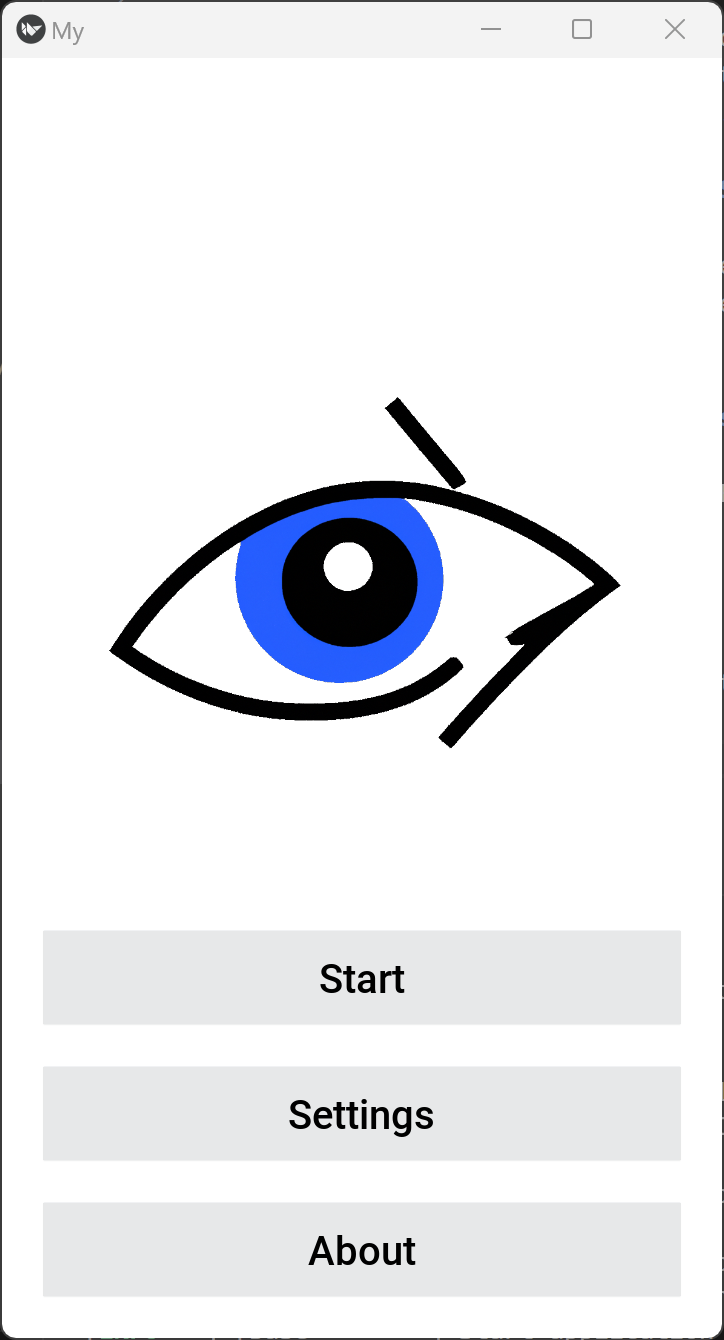
\includegraphics[width=\linewidth]{images/mainscreen.png}
		\caption{}
		\label{fig:mainscreen}
	\end{minipage}
	\hfill
	\begin{minipage}[b]{0.22\textwidth}
		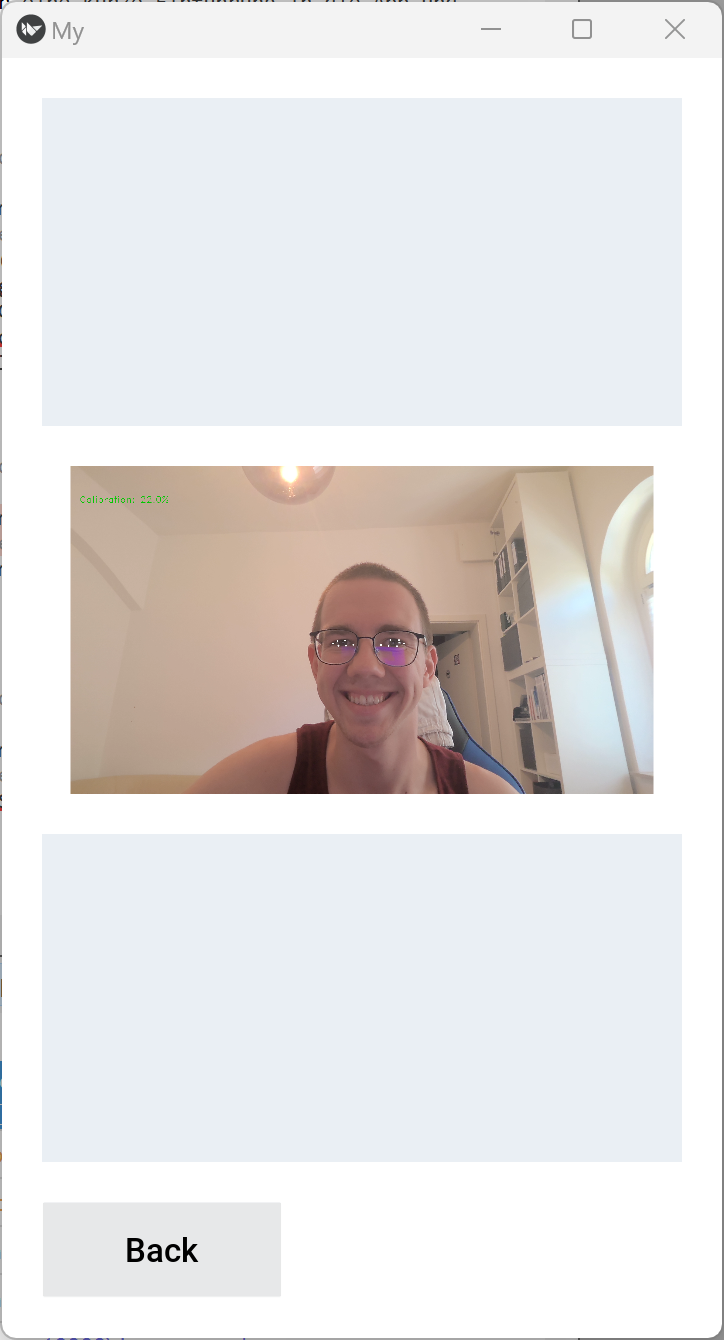
\includegraphics[width=\linewidth]{images/detectionscreen.png}
		\caption{}
		\label{fig:detectionscreen}
	\end{minipage}
	\hfill
	\begin{minipage}[b]{0.22\textwidth}
		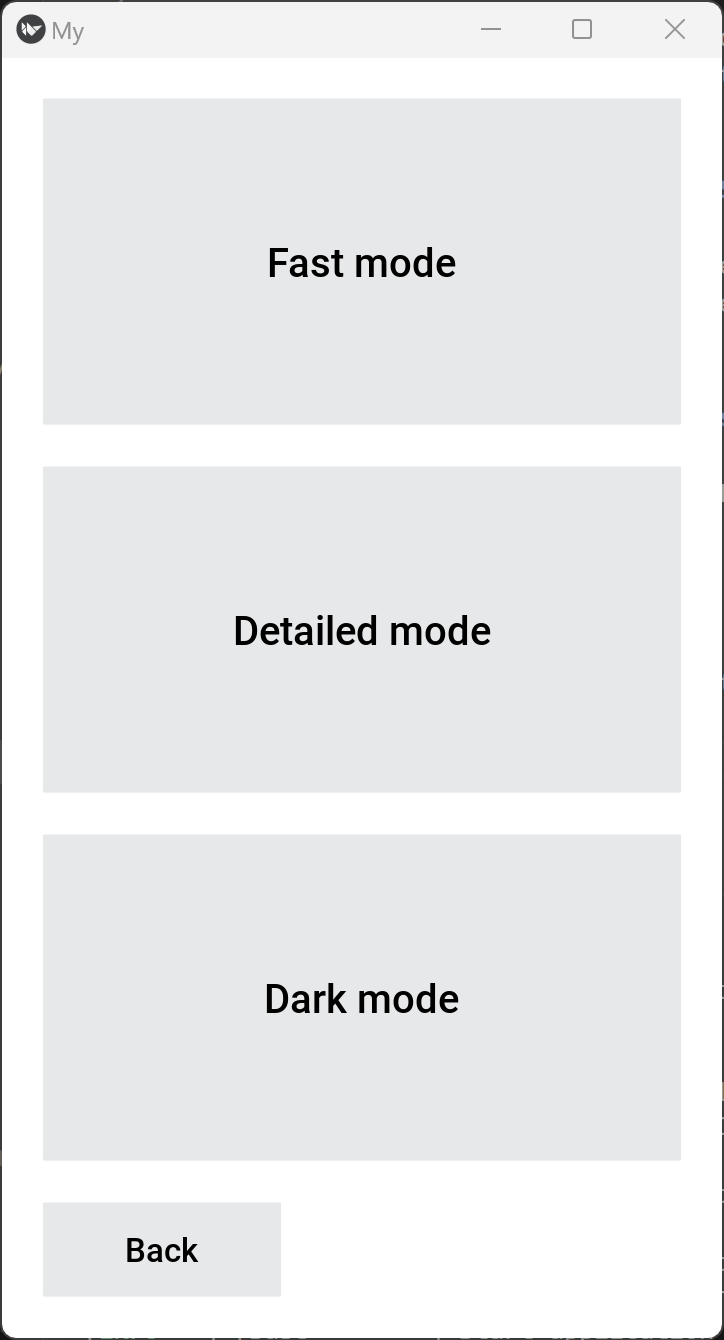
\includegraphics[width=\linewidth]{images/settingscreen.png}
		\caption{}
		\label{fig:settingscreen}
	\end{minipage}
	\hfill
	\begin{minipage}[b]{0.22\textwidth}
		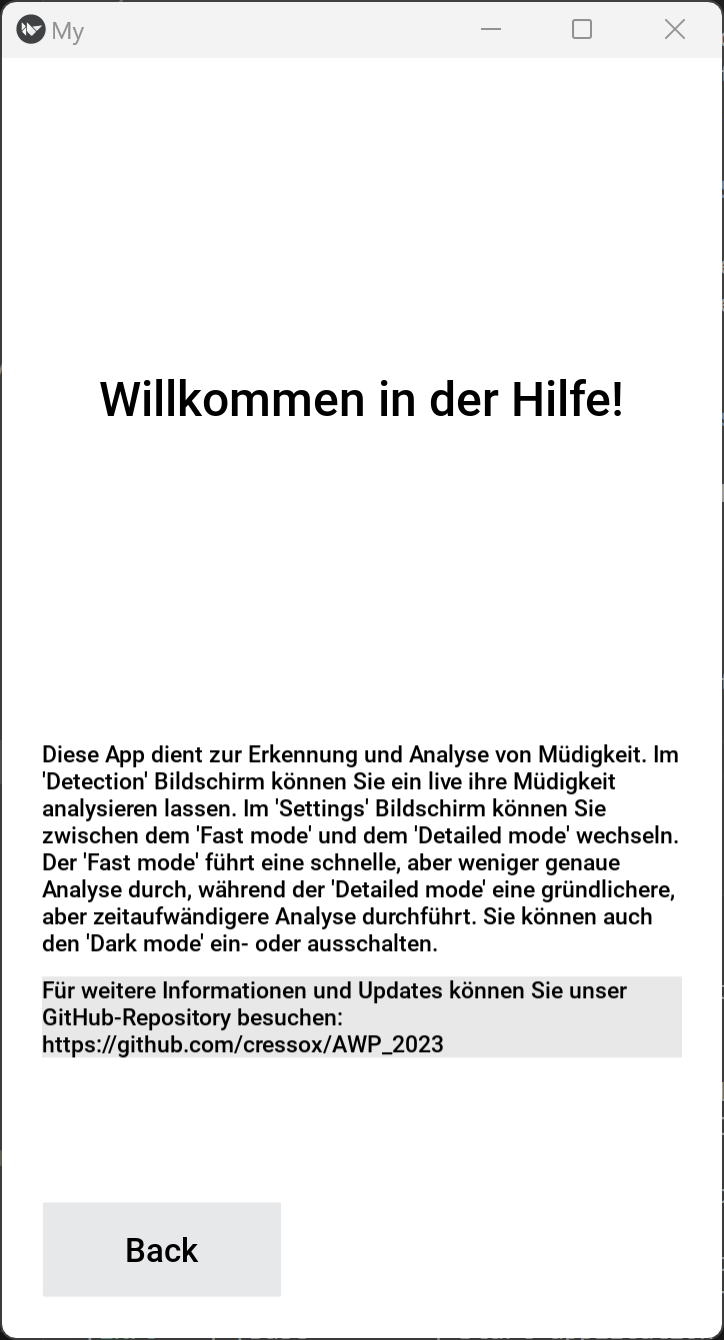
\includegraphics[width=\linewidth]{images/helpscreen.png}
		\caption{}
		\label{fig:helpscreen}
	\end{minipage}
\end{figure}

In Abbildung \ref{fig:mainscreen} ist der Einstiegsbildschirm der App zu sehen. Hier erhalten Benutzer eine kurze Einführung in die App und können die Müdigkeitserkennung starten oder auf die Einstellungen zugreifen. Die eigentliche Müdigkeitserkennung findet im Erkennungsbildschirm (Abbildung \ref{fig:detectionscreen}) statt, wo erkannte Gesichtsmerkmale wie die Augen markiert werden. Bei Erkennung von Müdigkeitsmerkmalen kann die App Warnungen anzeigen oder Alarmtöne abspielen. Im Einstellungsbildschirm (Abbildung \ref{fig:settingscreen}) können Benutzer verschiedene Einstellungen für die Benutzeroberfläche anpassen. Der Hilfebildschirm (Abbildung \ref{fig:helpscreen}) bietet detaillierte Informationen zur Verwendung der App und ihrer Funktionen.
